\documentclass[12pt,a4paper]{article}

\usepackage{fancyhdr}
\usepackage{graphicx}
\usepackage{placeins}
\usepackage{adjustbox}


\begin{document}

\pagestyle{fancy}
\fancyhf{}
\chead{Short summary report}

\begin{table}[t]
\centering
\caption {rnaQUAST metrics for assembled transcripts. In each row the best values are indicated with \textbf{bold}. For the transcript metrics (rows 4, 5, 6, 9, 13, 26, 27, 28) we highlighted the best \textbf{relative} values i.e. divided by the total number of transcripts in the corresponding assembly.}
\begin{adjustbox}{width=1\textwidth}
\small
\begin{tabular}{|l*{11}{|r}|}
\hline
\textbf{METRICS/TRANSCRIPTS}                            & \textbf{Trinity}       & \textbf{Trans-ABySS}   & \textbf{Oases}         & \textbf{SOAPdenovo-Trans} & \textbf{IDBA-Tran}     & \textbf{Bridger}       & \textbf{BinPacker}     & \textbf{Shannon}       & \textbf{rnaSPAdes}     & \textbf{SPAdes}        \\ \hline\hline
\multicolumn{11}{l}{\bf DATABASE METRICS}                                                 \\ \hline
Genes                                                   & 57992                  & 57992                  & 57992                  & 57992                  & 57992                  & 57992                  & 57992                  & 57992                  & 57992                  & 57992                  \\
Avg. number of exons per isoform                        & 5.971                  & 5.971                  & 5.971                  & 5.971                  & 5.971                  & 5.971                  & 5.971                  & 5.971                  & 5.971                  & 5.971                  \\ \hline
\multicolumn{11}{l}{\bf BASIC TRANSCRIPTS METRICS}                                        \\ \hline
Transcripts                                             & 96550                  & 227117                 & 218483                 & 132751                 & 75087                  & 82495                  & 1885                   & 103815                 & 197477                 & 85257                  \\
Transcripts $>$ 500 bp                                  & 41779                  & 56023                  & 141416                 & 23602                  & 29737                  & 32853                  & \textbf{1806}          & 45423                  & 30090                  & 23614                  \\
Transcripts $>$ 1000 bp                                 & 27154                  & 30767                  & 98196                  & 13110                  & 13508                  & 20434                  & \textbf{1646}          & 28248                  & 17195                  & 12775                  \\ \hline
\multicolumn{11}{l}{\bf ALIGNMENT METRICS}                                                \\ \hline
Aligned                                                 & 96414                  & 226264                 & 217524                 & 132192                 & 75016                  & 82359                  & 1876                   & \textbf{103729}        & 195967                 & 85001                  \\
Uniquely aligned                                        & 92154                  & 213998                 & 186940                 & 130119                 & 74003                  & 77699                  & 1489                   & 98368                  & 191228                 & 79356                  \\
Multiply aligned                                        & 554                    & 2151                   & 1224                   & 1360                   & 402                    & 441                    & 13                     & 565                    & 1543                   & 1612                   \\
Unaligned                                               & 136                    & 853                    & 959                    & 559                    & 71                     & 136                    & 9                      & \textbf{86}            & 1510                   & 256                    \\ \hline
\multicolumn{11}{l}{\bf ALIGNMENT METRICS FOR NON-MISASSEMBLED TRANSCRIPTS}               \\ \hline
Avg. aligned fraction                                   & 0.982                  & 0.974                  & 0.925                  & \textbf{0.993}         & 0.992                  & 0.978                  & 0.908                  & 0.982                  & 0.986                  & 0.983                  \\
Avg. alignment length                                   & 1083.555               & 517.916                & 1308.216               & 464.368                & 718.402                & 925.619                & \textbf{2899.392}      & 921.046                & 462.087                & 661.322                \\
Avg. mismatches per transcript                          & 1.728                  & 0.704                  & 2.383                  & \textbf{0.429}         & 0.799                  & 1.43                   & 6.184                  & 1.313                  & 1.001                  & 0.944                  \\ \hline
\multicolumn{11}{l}{\bf ALIGNMENT METRICS FOR MISASSEMBLED (CHIMERIC) TRANSCRIPTS}          \\ \hline
Misassemblies                                           & 1580                   & 7956                   & 24845                  & \textbf{148}           & 178                    & 1853                   & 279                    & 2161                   & 943                    & 1262                   \\ \hline
\multicolumn{11}{l}{\bf ASSEMBLY COMPLETENESS (SENSITIVITY)}                              \\ \hline
Database coverage                                       & 0.163                  & \textbf{0.19}          & 0.185                  & 0.145                  & 0.137                  & 0.135                  & 0.006                  & 0.149                  & 0.16                   & 0.132                  \\
50\%-assembled genes                                    & 9238                   & \textbf{9697}          & 9622                   & 8709                   & 8041                   & 8244                   & 453                    & 8147                   & 9604                   & 8849                   \\
95\%-assembled genes                                    & \textbf{3275}          & 2971                   & 3265                   & 2481                   & 569                    & 2540                   & 227                    & 2047                   & 3173                   & 2650                   \\
50\%-covered genes                                      & 10687                  & 11339                  & 10755                  & 10562                  & 10360                  & 9664                   & 458                    & 10039                  & \textbf{11370}         & 9988                   \\
95\%-covered genes                                      & 4162                   & 4144                   & \textbf{4303}          & 3195                   & 1639                   & 3066                   & 235                    & 3018                   & 4129                   & 3126                   \\
50\%-assembled isoforms                                 & 12986                  & 15150                  & \textbf{16278}         & 9932                   & 9681                   & 10020                  & 550                    & 11168                  & 11442                  & 9529                   \\
95\%-assembled isoforms                                 & 3826                   & 3153                   & \textbf{3948}          & 2553                   & 569                    & 2781                   & 255                    & 2303                   & 3335                   & 2653                   \\
50\%-covered isoforms                                   & 15216                  & \textbf{19670}         & 18656                  & 12582                  & 13221                  & 11907                  & 556                    & 14104                  & 14134                  & 11049                  \\
95\%-covered isoforms                                   & 4833                   & 4480                   & \textbf{5211}          & 3284                   & 1642                   & 3327                   & 264                    & 3403                   & 4338                   & 3132                   \\
Mean isoform coverage                                   & 0.518                  & 0.444                  & 0.549                  & 0.383                  & 0.454                  & 0.455                  & \textbf{0.718}         & 0.524                  & 0.407                  & 0.451                  \\
Mean isoform assembly                                   & 0.464                  & 0.38                   & 0.498                  & 0.332                  & 0.381                  & 0.408                  & \textbf{0.712}         & 0.45                   & 0.354                  & 0.407                  \\ \hline
\multicolumn{11}{l}{\bf GeneMarkS-T METRICS}                                              \\ \hline
Predicted genes                                         & 30445                  & 44205                  & \textbf{95194}         & 16217                  & 23025                  & 22024                  & 1376                   & 35683                  & 20358                  & 15761                  \\ \hline
\multicolumn{11}{l}{\bf ASSEMBLY SPECIFICITY}                                             \\ \hline
50\%-matched                                            & 53868                  & 112373                 & 131790                 & 58860                  & 45371                  & 42711                  & 1269                   & \textbf{71978}         & 58962                  & 35654                  \\
95\%-matched                                            & 36225                  & 75135                  & 69556                  & 49648                  & 38273                  & 30697                  & 595                    & \textbf{56189}         & 42860                  & 27474                  \\
Unannotated                                             & 31271                  & 88770                  & 37816                  & 61115                  & 22079                  & 27369                  & \textbf{86}            & 22475                  & 120552                 & 39000                  \\
Mean fraction of transcript matched                     & 0.555                  & 0.49                   & 0.645                  & 0.441                  & 0.602                  & 0.529                  & \textbf{0.769}         & 0.698                  & 0.298                  & 0.41                   \\ \hline
\end{tabular}
\end{adjustbox}
\end{table}

\FloatBarrier
\clearpage
\lfoot{generated by rnaQUAST}

\begin{figure}[t]
\centering
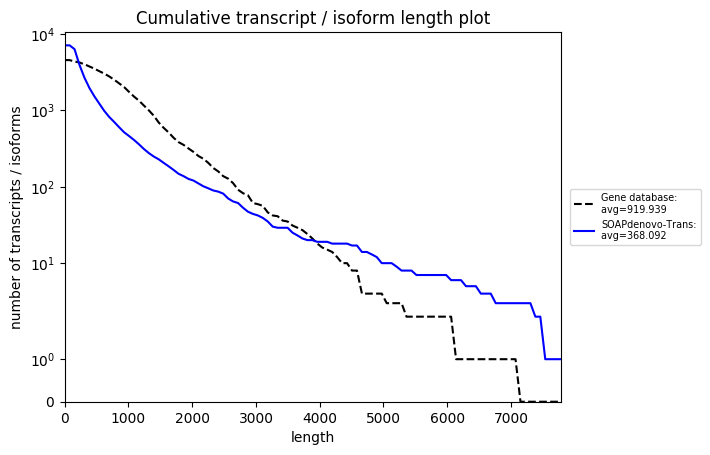
\includegraphics[width = \linewidth]{/mnt/dessertlocal/projects/transcriptome_assembly/review/evaluation/rna-quast/ebov_hsa_3h/comparison_output/transcript_length.png}
\caption{Plot showing cumulative transcript length distribution. Each point represents the number of transcripts in the assembly with the corresponding length or longer; black dashed line corresponds to the database isoforms; the plot is given in logarithmic scale.}
\end{figure}
\FloatBarrier
\clearpage


\begin{figure}[t]
\centering
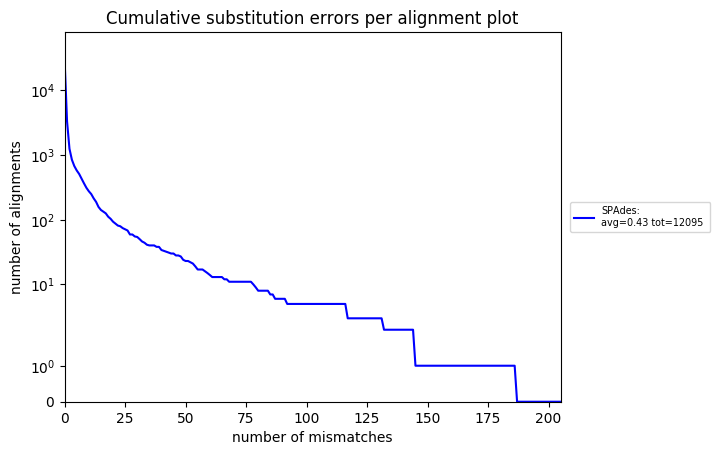
\includegraphics[width = \linewidth]{/mnt/dessertlocal/projects/transcriptome_assembly/review/evaluation/rna-quast/ebov_hsa_3h/comparison_output/mismatch_rate.png}
\caption{Plot showing cumulative substitution errors per alignment distribution. Each point represents the number of alignments with the corresponding number of mismatches or greater; the plot is given in logarithmic scale.}
\end{figure}
\FloatBarrier
\clearpage


\begin{figure}[t]
\centering
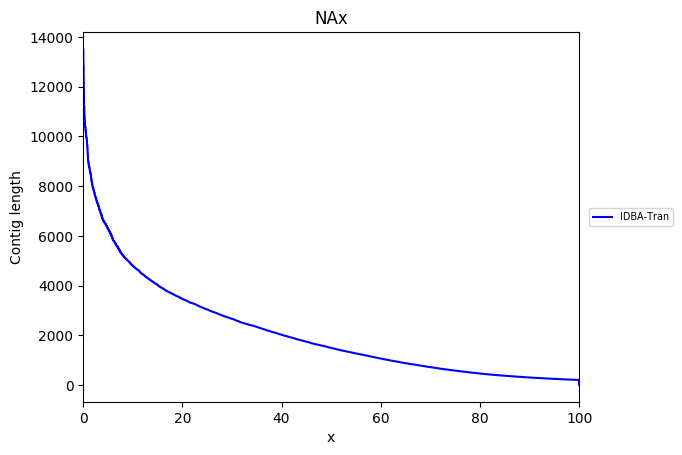
\includegraphics[width = \linewidth]{/mnt/dessertlocal/projects/transcriptome_assembly/review/evaluation/rna-quast/ebov_hsa_3h/comparison_output/NAx.png}
\caption{Nx plot for transcripts. Nx is a maximal number $N$, such that the total length of all transcripts longer than $N$ bp is at least $x\%$ of the total length of all transcripts.}
\end{figure}
\FloatBarrier
\clearpage


\begin{figure}[t]
\centering
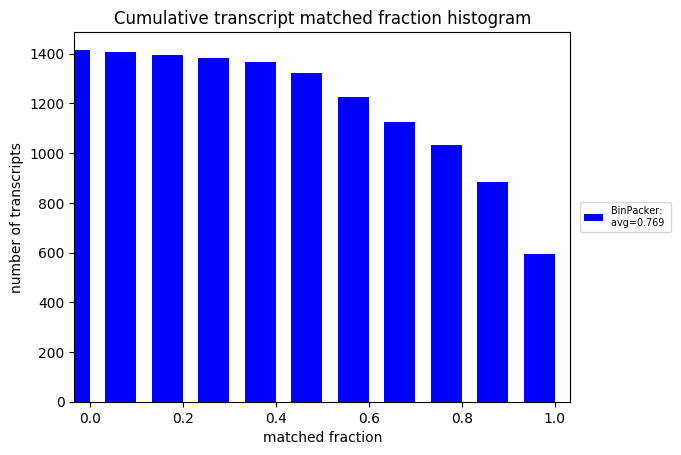
\includegraphics[width = \linewidth]{/mnt/dessertlocal/projects/transcriptome_assembly/review/evaluation/rna-quast/ebov_hsa_3h/comparison_output/x-matched.png}
\caption{Plot showing cumulative transcript match histogram. Each bar represents the number of transcripts with matched fraction equal to or greater than the value on $x$ axis; transcript matched fraction is calculated as the number of its bases covering an isoform divided by the transcript length.}
\end{figure}
\FloatBarrier
\clearpage


\begin{figure}[t]
\centering
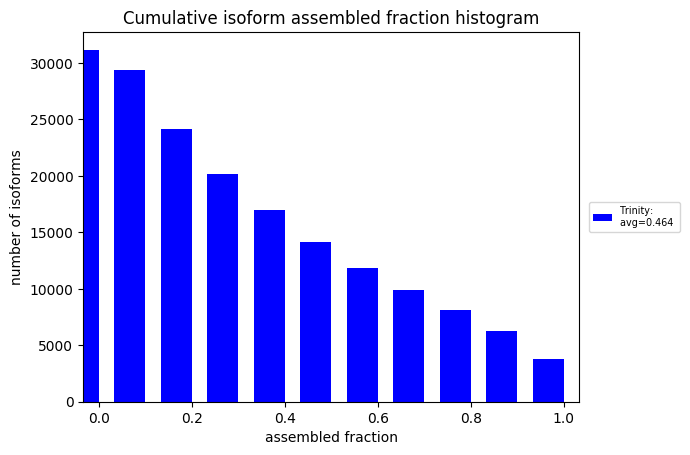
\includegraphics[width = \linewidth]{/mnt/dessertlocal/projects/transcriptome_assembly/review/evaluation/rna-quast/ebov_hsa_3h/comparison_output/x-assembled.png}
\caption{Plot showing cumulative isoform assembly histogram. Each bar represents the number of isoforms with assembled fraction equal to or greater than the value on $x$ axis; isoform assembled fraction is calculated as the maximum number of captured by single assembled transcript bases divided by the total isoform length.}
\end{figure}
\FloatBarrier
\clearpage


\begin{figure}[t]
\centering
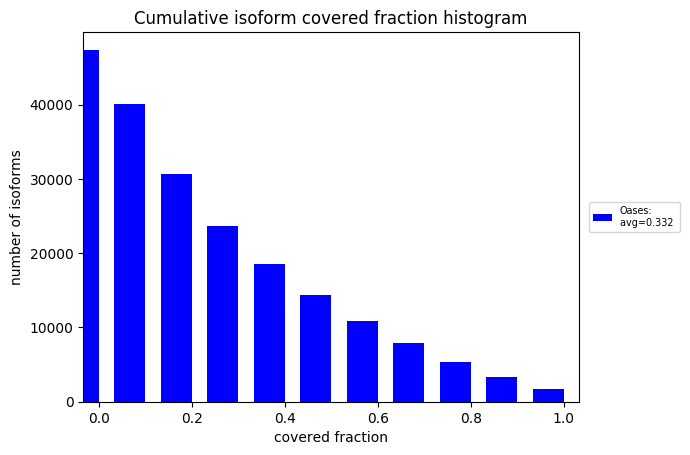
\includegraphics[width = \linewidth]{/mnt/dessertlocal/projects/transcriptome_assembly/review/evaluation/rna-quast/ebov_hsa_3h/comparison_output/x-covered.png}
\caption{Plot showing cumulative isoform coverage histogram. Each bar represents the number of isoforms with covered fraction equal to or greater than the value on $x$ axis; isoform covered fraction is calculated as the number of covered bases (by all transcripts in the assembly) divided by the total isoform length.}
\end{figure}
\FloatBarrier
\clearpage


\end{document}
